\documentclass[esp]{SpeedEstimationAI_paper}
\usepackage{authblk}

%
% Publication Title
\title{Reconstrucción Forense de Velocidad Vehicular Preimpacto mediante Redes Neuronales Convolucionales y Modelado de Deformación Estructural Postcolisión}

% Short title for the header (copy the main title if it is not too long)
\shorttitle{Reconstrucción de Velocidad Vehicular}
       
% Authors
\author[1]{Alberto Isaac Sánchez Tarango}
\author[1]{Alyson Melissa Sánchez Serratos}
\author[1]{Máximo Moises Zamudio Chávez}
\author[1]{Miguel Ángel Pérez Ávila}
\author[1]{Santiago Albarrán Organista}
\author[1]{Víctor Alonzo Estévez Chávez}

% Author Affiliations
\affil[1]{Tecnológico de Monterrey, Escuela de Ingeniería y Ciencias, Campus Toluca, Estado de México, México}

% Surname of the first author of the manuscript
\firstauthor{Sánchez, Sánchez, Zamudio}

%Contact Author Information
\contactauthor{Alberto Sánchez}           % Name and surname of the contact author
\email{A01771321@tec.mx}                                  % Contact Author Email

% Publication data (will be defined in the edition)
\thisvolume{XX}
\thisnumber{XX}
\thismonth{Month}
\thisyear{20XX}
\receptiondate{dd/mm/aaaa}
\acceptancedate{dd/mm/aaaa}
\publicationdate{dd/mm/aaaa}

% Place your particular definitions here
\newcommand{\vect}[1]{\mathbf{#1}}  % vectors

% Insert here the abstract in English language
\abstract{
Lorem ipsum dolor sit amet, consectetur adipiscing elit, sed do eiusmod tempor incididunt ut labore et dolore magna aliqua. Ut enim ad minim veniam, quis nostrud exercitation ullamco laboris nisi ut aliquip ex ea commodo consequat. Duis aute irure dolor in reprehenderit in voluptate velit esse cillum dolore eu fugiat nulla pariatur. Excepteur sint occaecat cupidatat non proident, sunt in culpa qui officia deserunt mollit anim id est laborum. Sed ut perspiciatis unde omnis iste natus error sit voluptatem accusantium doloremque laudantium, totam rem aperiam.}

% Insert here the keywords of your work in English language
\keywords{
Lorem ipsum, dolor sit amet, consectetur adipiscing, eiusmod tempor, labore et dolore}

% Insert here the abstract in Spanish language
\resumen{
Lorem ipsum dolor sit amet, consectetur adipiscing elit, sed do eiusmod tempor incididunt ut labore et dolore magna aliqua. Ut enim ad minim veniam, quis nostrud exercitation ullamco laboris nisi ut aliquip ex ea commodo consequat. Duis aute irure dolor in reprehenderit in voluptate velit esse cillum dolore eu fugiat nulla pariatur. Excepteur sint occaecat cupidatat non proident, sunt in culpa qui officia deserunt mollit anim id est laborum. Sed ut perspiciatis unde omnis iste natus error sit voluptatem accusantium doloremque laudantium, totam rem aperiam.}

% Insert here the keywords of your work in Spanish language
\palabrasclave{
reconstrucción forense, estimación de velocidad de impacto, visión por computadora, redes neuronales convolucionales, aprendizaje por transferencia, deformación estructural}

% Roman numerals for section numbering
\renewcommand{\thesection}{\Roman{section}}

% Start document
\begin{document}

% Include title, authors, abstract, etc.
\maketitle
\thispagestyle{fancy}
\printcontactdata

\section{INTRODUCCIÓN}

\firstword{L}{os} siniestros viales representan una de las principales problemáticas contemporáneas en materia de salud pública, seguridad vial y pérdidas económicas. La Organización Mundial de la Salud estima que aproximadamente 1.19 millones de personas fallecen anualmente como consecuencia de accidentes de tránsito, mientras que decenas de millones sufren lesiones permanentes o discapacidades asociadas \cite{WHO_RoadTrafficInjuries}. Más allá de su impacto humano, estos eventos generan costos sustanciales para los sistemas de salud, los marcos regulatorios y el sector asegurador, particularmente en los procesos de reconstrucción técnica y determinación de responsabilidades.

En el ámbito de la ingeniería forense automotriz, la estimación de la velocidad de impacto constituye uno de los parámetros más relevantes para la reconstrucción de colisiones. Dicho parámetro permite inferir la severidad energética del evento, validar trayectorias de movimiento y respaldar técnicamente dictámenes periciales y procedimientos judiciales. Tradicionalmente, estas estimaciones se fundamentan en modelos físico--mecánicos basados en conservación del momento, disipación de energía y análisis de deformación estructural, consolidados históricamente en metodologías como CRASH3, el Método McHenry y diversos modelos de \textit{crush energy analysis} \cite{FrickeTrafficCrashReconstruction,BrachBrach2011,DailyShigemura2020}. Tales enfoques han demostrado alta utilidad en contextos especializados; sin embargo, su aplicación depende de inspecciones presenciales exhaustivas, mediciones geométricas precisas y acceso directo a las zonas deformadas del vehículo.

A pesar de su robustez teórica, los métodos convencionales presentan limitaciones importantes en escenarios reales de reconstrucción. La evidencia física suele encontrarse incompleta, alterada por maniobras de rescate o degradada por condiciones ambientales posteriores al impacto. Asimismo, la obtención de parámetros de rigidez vehicular y deformación residual requiere instrumentación especializada y personal altamente capacitado, lo que incrementa significativamente los costos operativos y la variabilidad interperito \cite{DailyShigemura2020}. En consecuencia, la reproducibilidad de los análisis puede verse comprometida cuando únicamente se dispone de evidencia parcial o documentación fotográfica del siniestro. Estas limitaciones han motivado el interés por metodologías alternativas capaces de aprovechar evidencia visual disponible incluso en ausencia de inspecciones físicas completas.

Paralelamente, la digitalización progresiva de expedientes periciales y la expansión de repositorios de accidentes reales han incrementado de manera sustancial la disponibilidad de imágenes postcolisión. Iniciativas como el \textit{Crash Injury Research and Engineering Network} (CIREN), desarrollado por la National Highway Traffic Safety Administration (NHTSA), integran investigaciones multidisciplinarias que incluyen fotografías vehiculares, reconstrucción técnica del accidente, variables biomecánicas y estimaciones de velocidad \cite{NHTSA_CIREN,Digges2005CIREN}. Este tipo de bases de datos constituye una oportunidad relevante para el desarrollo de metodologías automatizadas capaces de inferir variables dinámicas de preimpacto a partir de evidencia visual estructurada.

En consonancia con esta creciente disponibilidad de evidencia visual, la literatura reciente en visión por computadora aplicada al sector automotriz se ha concentrado principalmente en detección de daños, clasificación de severidad y automatización de reclamaciones aseguradoras. No obstante, la estimación cuantitativa de velocidad de impacto a partir de imágenes posteriores a la colisión continúa siendo un problema relativamente poco explorado en comparación con otras tareas de análisis vehicular. Aunque actualmente existen datasets y enfoques orientados a análisis de daños, numerosos métodos continúan dependiendo de variables físicas adicionales, mediciones manuales o parámetros estructurales difíciles de obtener fuera de entornos controlados \cite{FrickeTrafficCrashReconstruction,BrachBrach2011}. Asimismo, la heterogeneidad visual de los escenarios reales de accidente y la variabilidad en la calidad de la evidencia fotográfica representan desafíos importantes para la generalización de modelos automatizados.

En este contexto, el presente trabajo propone una metodología de reconstrucción de velocidad vehicular preimpacto basada exclusivamente en imágenes de siniestros y técnicas de aprendizaje profundo. Inicialmente, se desarrolla un pipeline reproducible de adquisición, validación y curación de datos utilizando casos provenientes de CIREN, incorporando procesos automatizados de filtrado visual, validación semántica y estructuración de metadatos. A partir de ello, se construye un conjunto de datos estandarizado con imágenes vehiculares y etiquetas de velocidad apto para entrenamiento supervisado de modelos de regresión.

Posteriormente, se plantea un esquema de aprendizaje basado en transferencia de conocimiento mediante arquitecturas convolucionales profundas. Se evalúan estrategias de \textit{Transfer Learning} y \textit{Knowledge Distillation} con el objetivo de mejorar la capacidad de generalización del modelo y reducir simultáneamente los requerimientos computacionales para escenarios de implementación práctica.

En síntesis, las contribuciones de este estudio son: (i) la sistematización de un proceso reproducible de preparación de datos forenses vehiculares con velocidades verificadas, (ii) la construcción de un dataset curado de siniestros reales orientado a estimación continua de velocidad y (iii) la propuesta de un modelo de aprendizaje profundo para reconstrucción automatizada de velocidad de impacto a partir de evidencia fotográfica. Estas aportaciones buscan avanzar hacia metodologías periciales más objetivas, escalables y consistentes, fortaleciendo el uso de inteligencia artificial en reconstrucción forense y análisis de colisiones viales.

\section{TRABAJO RELACIONADO}

La estimación automática de velocidad vehicular mediante visión por computadora ha recibido creciente atención en los últimos años debido a su relevancia en sistemas inteligentes de transporte, conducción autónoma y reconstrucción forense de accidentes. Los enfoques recientes se han apoyado principalmente en aprendizaje profundo, análisis geométrico y procesamiento de video monocular para inferir velocidad a partir de imágenes o secuencias visuales.

En el contexto de sistemas ADAS y monitoreo vehicular, García-Aguilar et al. \cite{Garcia2024Speed} propusieron un framework de estimación de velocidad en tiempo real basado en redes neuronales convolucionales y cámaras monoculares. Su metodología combina detección de vehículos, estimación de profundidad y seguimiento visual para calcular la velocidad relativa de vehículos circundantes en entornos urbanos simulados mediante CARLA. Los autores reportaron errores promedio inferiores a 3 km/h en múltiples escenarios de tráfico, demostrando que arquitecturas profundas pueden inferir variables dinámicas relevantes únicamente a partir de información visual.

De forma complementaria, Macko et al. \cite{Macko2025Speed} desarrollaron un enfoque eficiente de estimación de velocidad basado en video monocular y geometría de perspectiva. Su propuesta integra detección profunda de vehículos con calibración automática de cámara y análisis tridimensional de trayectorias, alcanzando errores relativos menores al 5\% en escenarios reales de tráfico urbano. El trabajo resulta relevante debido a que demuestra la viabilidad de inferir velocidad utilizando únicamente información visual sin necesidad de sensores especializados adicionales.

En el ámbito específico de reconstrucción forense, Silver et al. \cite{Silver2022CrashCharacteristics} presentaron uno de los primeros trabajos orientados a estimar características de colisión a partir de imágenes de vehículos accidentados utilizando aprendizaje profundo. Su estudio empleó redes neuronales convolucionales para predecir variables asociadas al impacto, incluyendo Delta-V y severidad de colisión, utilizando fotografías postcolisión provenientes de accidentes reales. Los resultados mostraron correlaciones significativas entre patrones visuales de deformación y parámetros dinámicos del accidente, sugiriendo que la evidencia fotográfica contiene información suficiente para inferir características físicas relevantes del impacto.

A pesar de estos avances, persisten desafíos importantes asociados a la heterogeneidad visual de los escenarios reales de accidente, variaciones de iluminación, ángulos de captura y calidad de evidencia fotográfica. Además, una parte importante de los trabajos recientes depende de secuencias de video, calibración geométrica o información contextual adicional, mientras que la estimación de velocidad exclusivamente a partir de imágenes postcolisión continúa siendo un área relativamente poco explorada.

\section{METODOLOGÍA}
Lorem ipsum dolor sit amet, consectetur adipiscing elit. Integer nec odio. Praesent libero. Sed cursus ante dapibus diam. Sed nisi. Nulla quis sem at nibh elementum imperdiet. Duis sagittis ipsum. Praesent mauris. Fusce nec tellus sed augue semper porta.

Mauris massa. Vestibulum lacinia arcu eget nulla. Class aptent taciti sociosqu ad litora torquent per conubia nostra, per inceptos himenaeos. Curabitur sodales ligula in libero. Sed dignissim lacinia nunc. Curabitur tortor.

Pellentesque nibh. Aenean quam. In scelerisque sem at dolor. Maecenas mattis. Sed convallis tristique sem. Proin ut ligula vel nunc egestas porttitor. Morbi lectus risus, iaculis vel, suscipit quis, luctus non, massa.

\subsection{Datos y preprocesamiento}
\subsubsection{Fuente de datos y criterios de construcción de la base de datos utilizada para el entrenamiento de los modelos predictivos de regresión}

La serie de componentes que han sido elaborados sobre la base de datos denominada \texttt{Crash Injury Research Engineering Network} (CIREN) y perteneciente al \texttt{NHTSA Crash Viewer}, se orientan a transformar información pública de siniestros vehiculares en una estructura analítica de importante utilidad para tareas de estimación de velocidad preimpacto a partir de evidencia postcolisión. Para ello, se parte de casos documentados con dos tipos de insumo complementario: metadatos del evento y del vehículo involucrado, junto con galerías fotográficas asociadas al daño observado tras la colisión. La lógica metodológica seguida no consiste únicamente en recolectar imágenes, sino en vincular cada fotografía válida con un contexto de siniestro suficientemente caracterizado en términos de severidad, dinámica de impacto y atributos generales del vehículo de tal manera que cada uno de estos elementos multimedia maximicen su valor cualitativo para la explicación del fenómeno físico de impacto y su relación directa con la velocidad a la que ocurrió.

El proceso se diseñó bajo tres principios: trazabilidad, reanudación y utilidad analítica. Primeramente, la trazabilidad garantiza que cada imagen final conserve su vínculo con el caso de origen y con el vehículo al que pertenece. Por otro lado, la reanudación permite continuar ejecuciones incompletas sin repetir el procesamiento ya realizado y, finalmente, la utilidad analítica asegura que el resultado no sea solo una galería visual, sino un conjunto estructurado de ejemplos listos para ser explorados y posteriormente consumidos por los modelos predictivos seleccionados.

\begin{figure}[htbp]
    \centering
    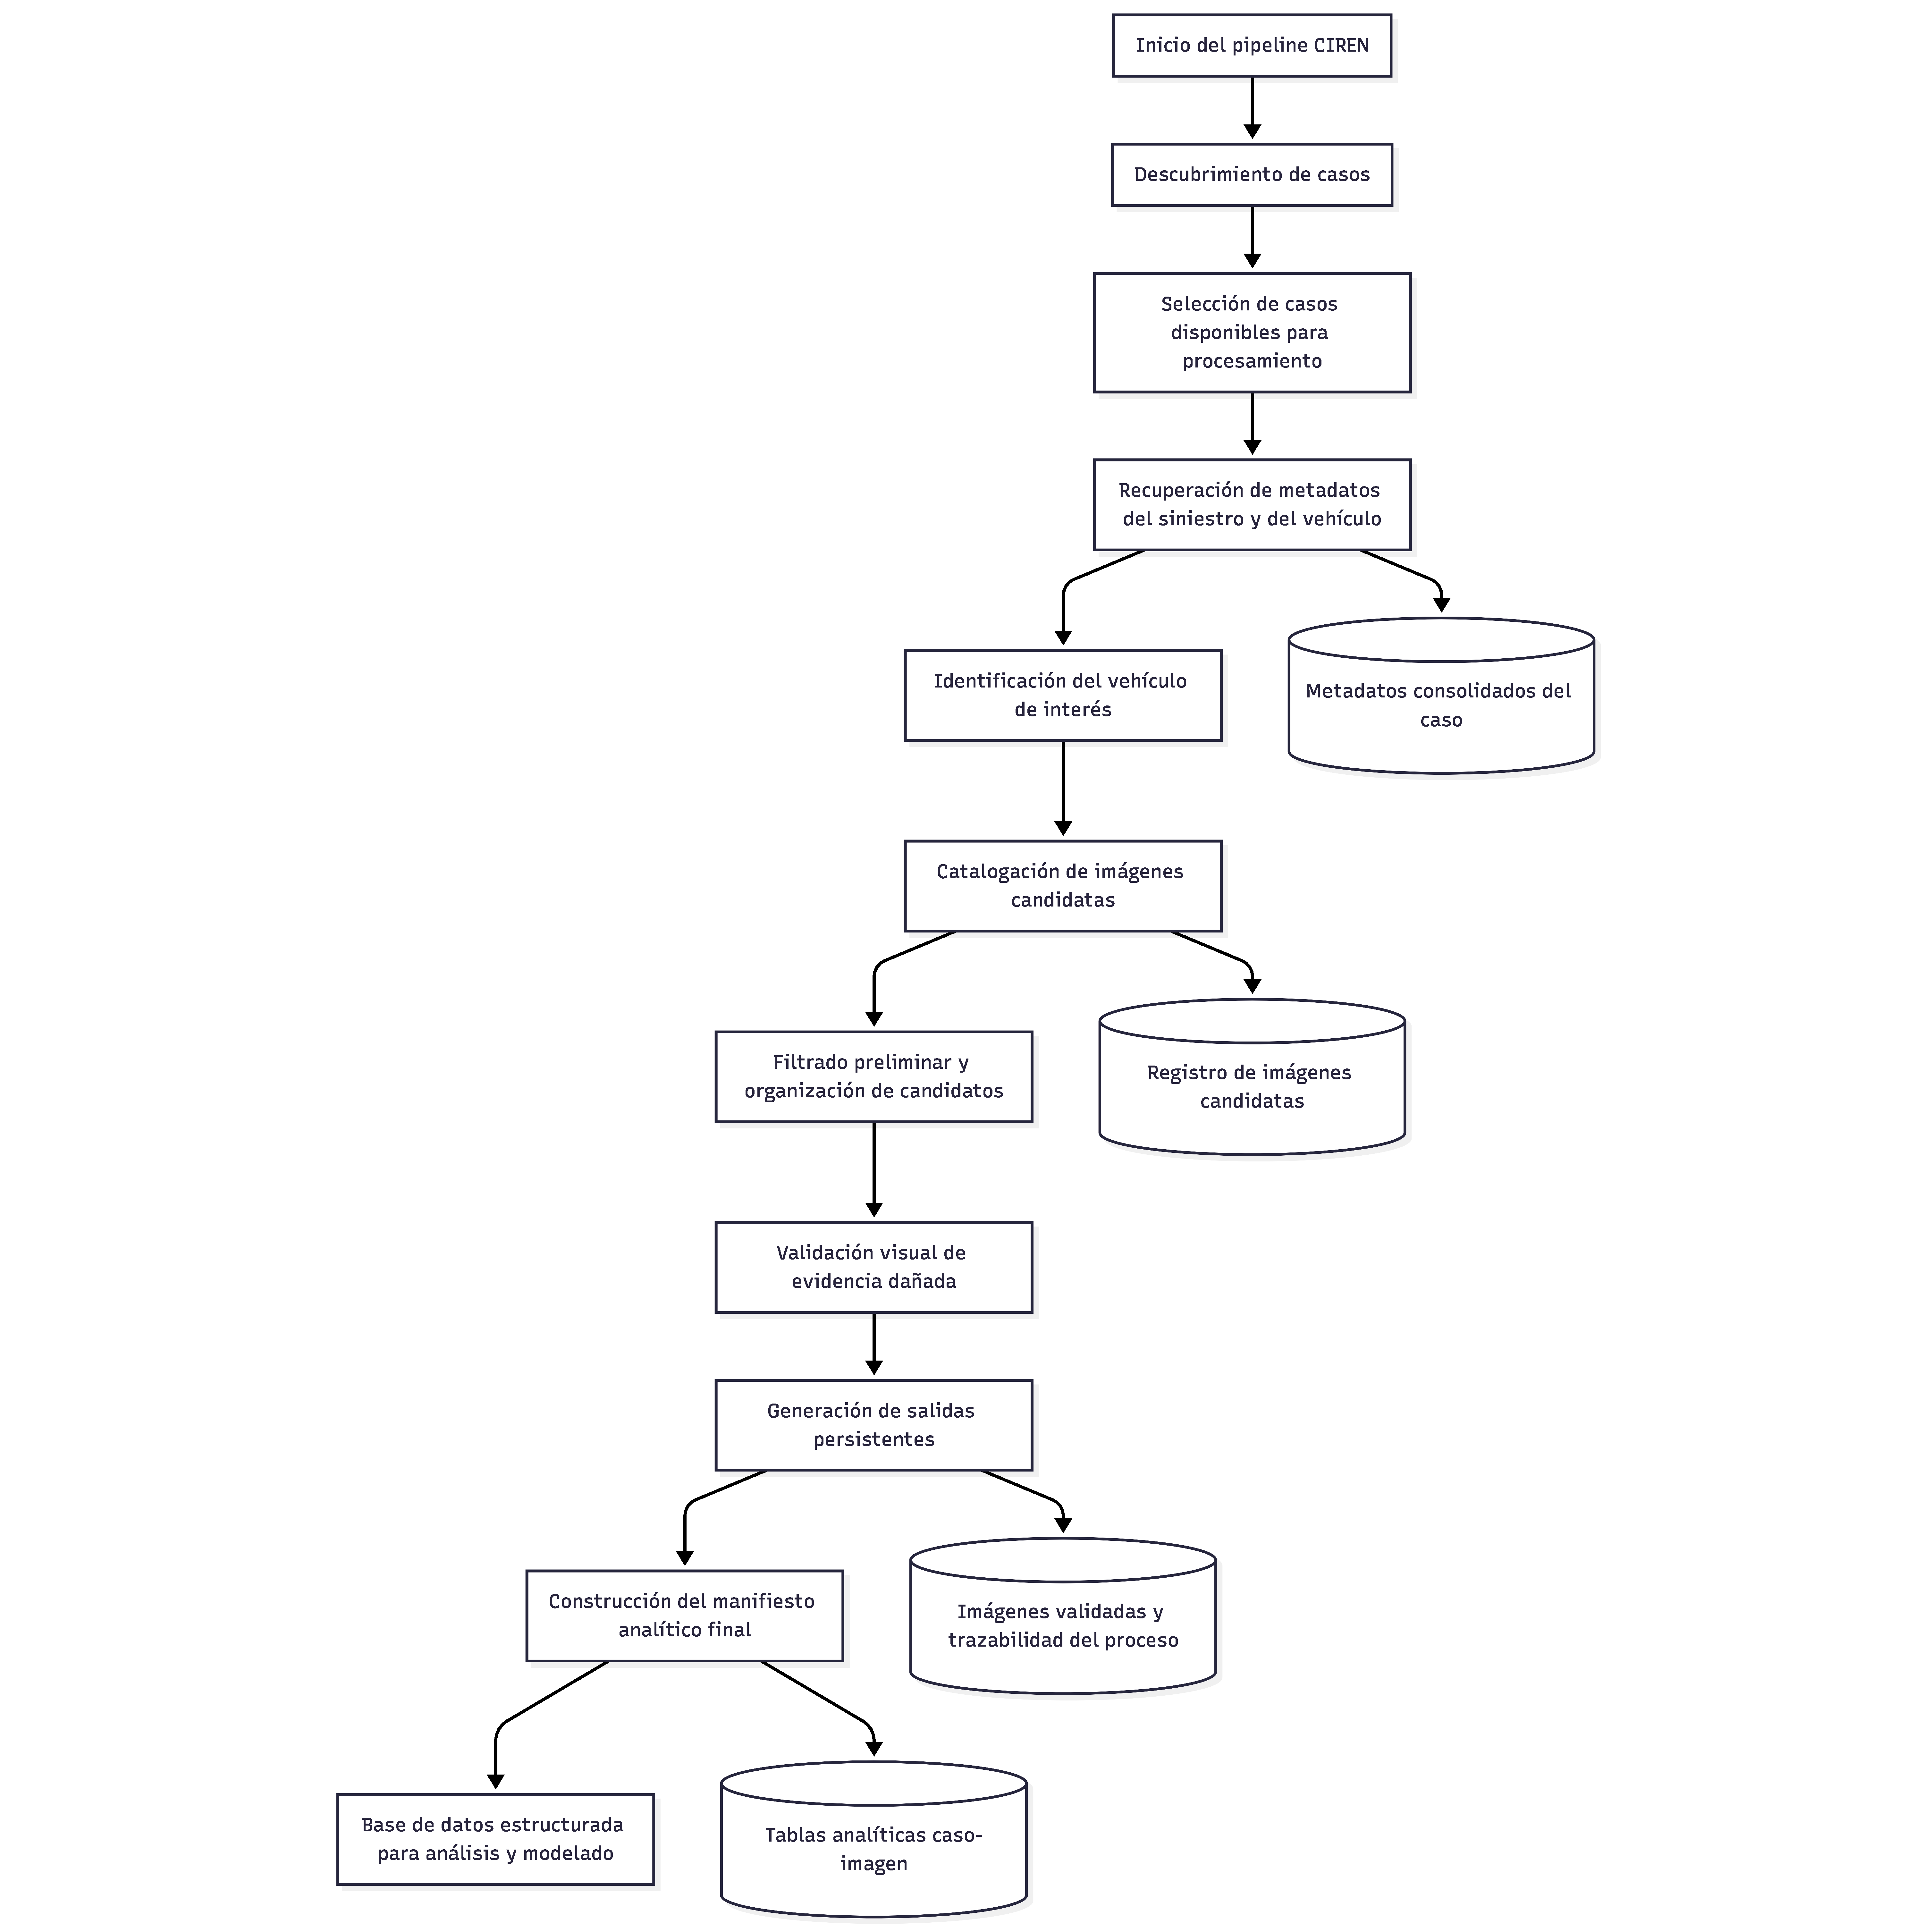
\includegraphics[width=\columnwidth]{Diagrams/Diagrama1.pdf}
    \caption{Diagrama de flujo general del pipeline para el tratamiento y persistencia de la base de datos de CIREN}
    \label{fig:diagrama1}
\end{figure}


\subsubsection{Caracterización del caso y selección del vehículo de interés}

Una vez identificado un caso particular desde la base de datos de \texttt{CIREN}, el flujo adquiere la responsabilidad de integrar la información descriptiva disponible para construir una representación compacta del evento. En esta etapa, se priorizan variables con valor directo para interpretación biomecánica y estructural del impacto tal y como lo son la severidad máxima de lesión humana tras el incidente, el cambio total de velocidad, la dirección del impacto, el patrón general de deformación, el plano principal de daño y características generales del vehículo, entre las cuales pueden ser encontradas: clase, masa base y carga reportada. Cada una de estas variables permiten contextualizar visualmente el daño y, al mismo tiempo, aportan atributos cuantitativos y categóricos relevantes para el diseño, preparación y entrenamiento de los modelos de inferencia.

Dado que un mismo caso puede contener múltiples vehículos o varias vistas de interés involucradas, se implementó una etapa de conciliación para identificar al vehículo principal que será estudiado. Esta decisión adquiere especial relevancia al permitir evitar la inadecuada mezcla de  imágenes pertenecientes a actores distintos dentro de un mismo siniestro, al igual que mejorar la coherencia entre la evidencia visual y los metadatos asociados. De esta forma, la unidad efectiva de análisis queda definida como el par compuesto por caso y vehículo principal, sobre el cual se organiza el resto del preprocesamiento.

\begin{figure}[htbp]
    \centering
    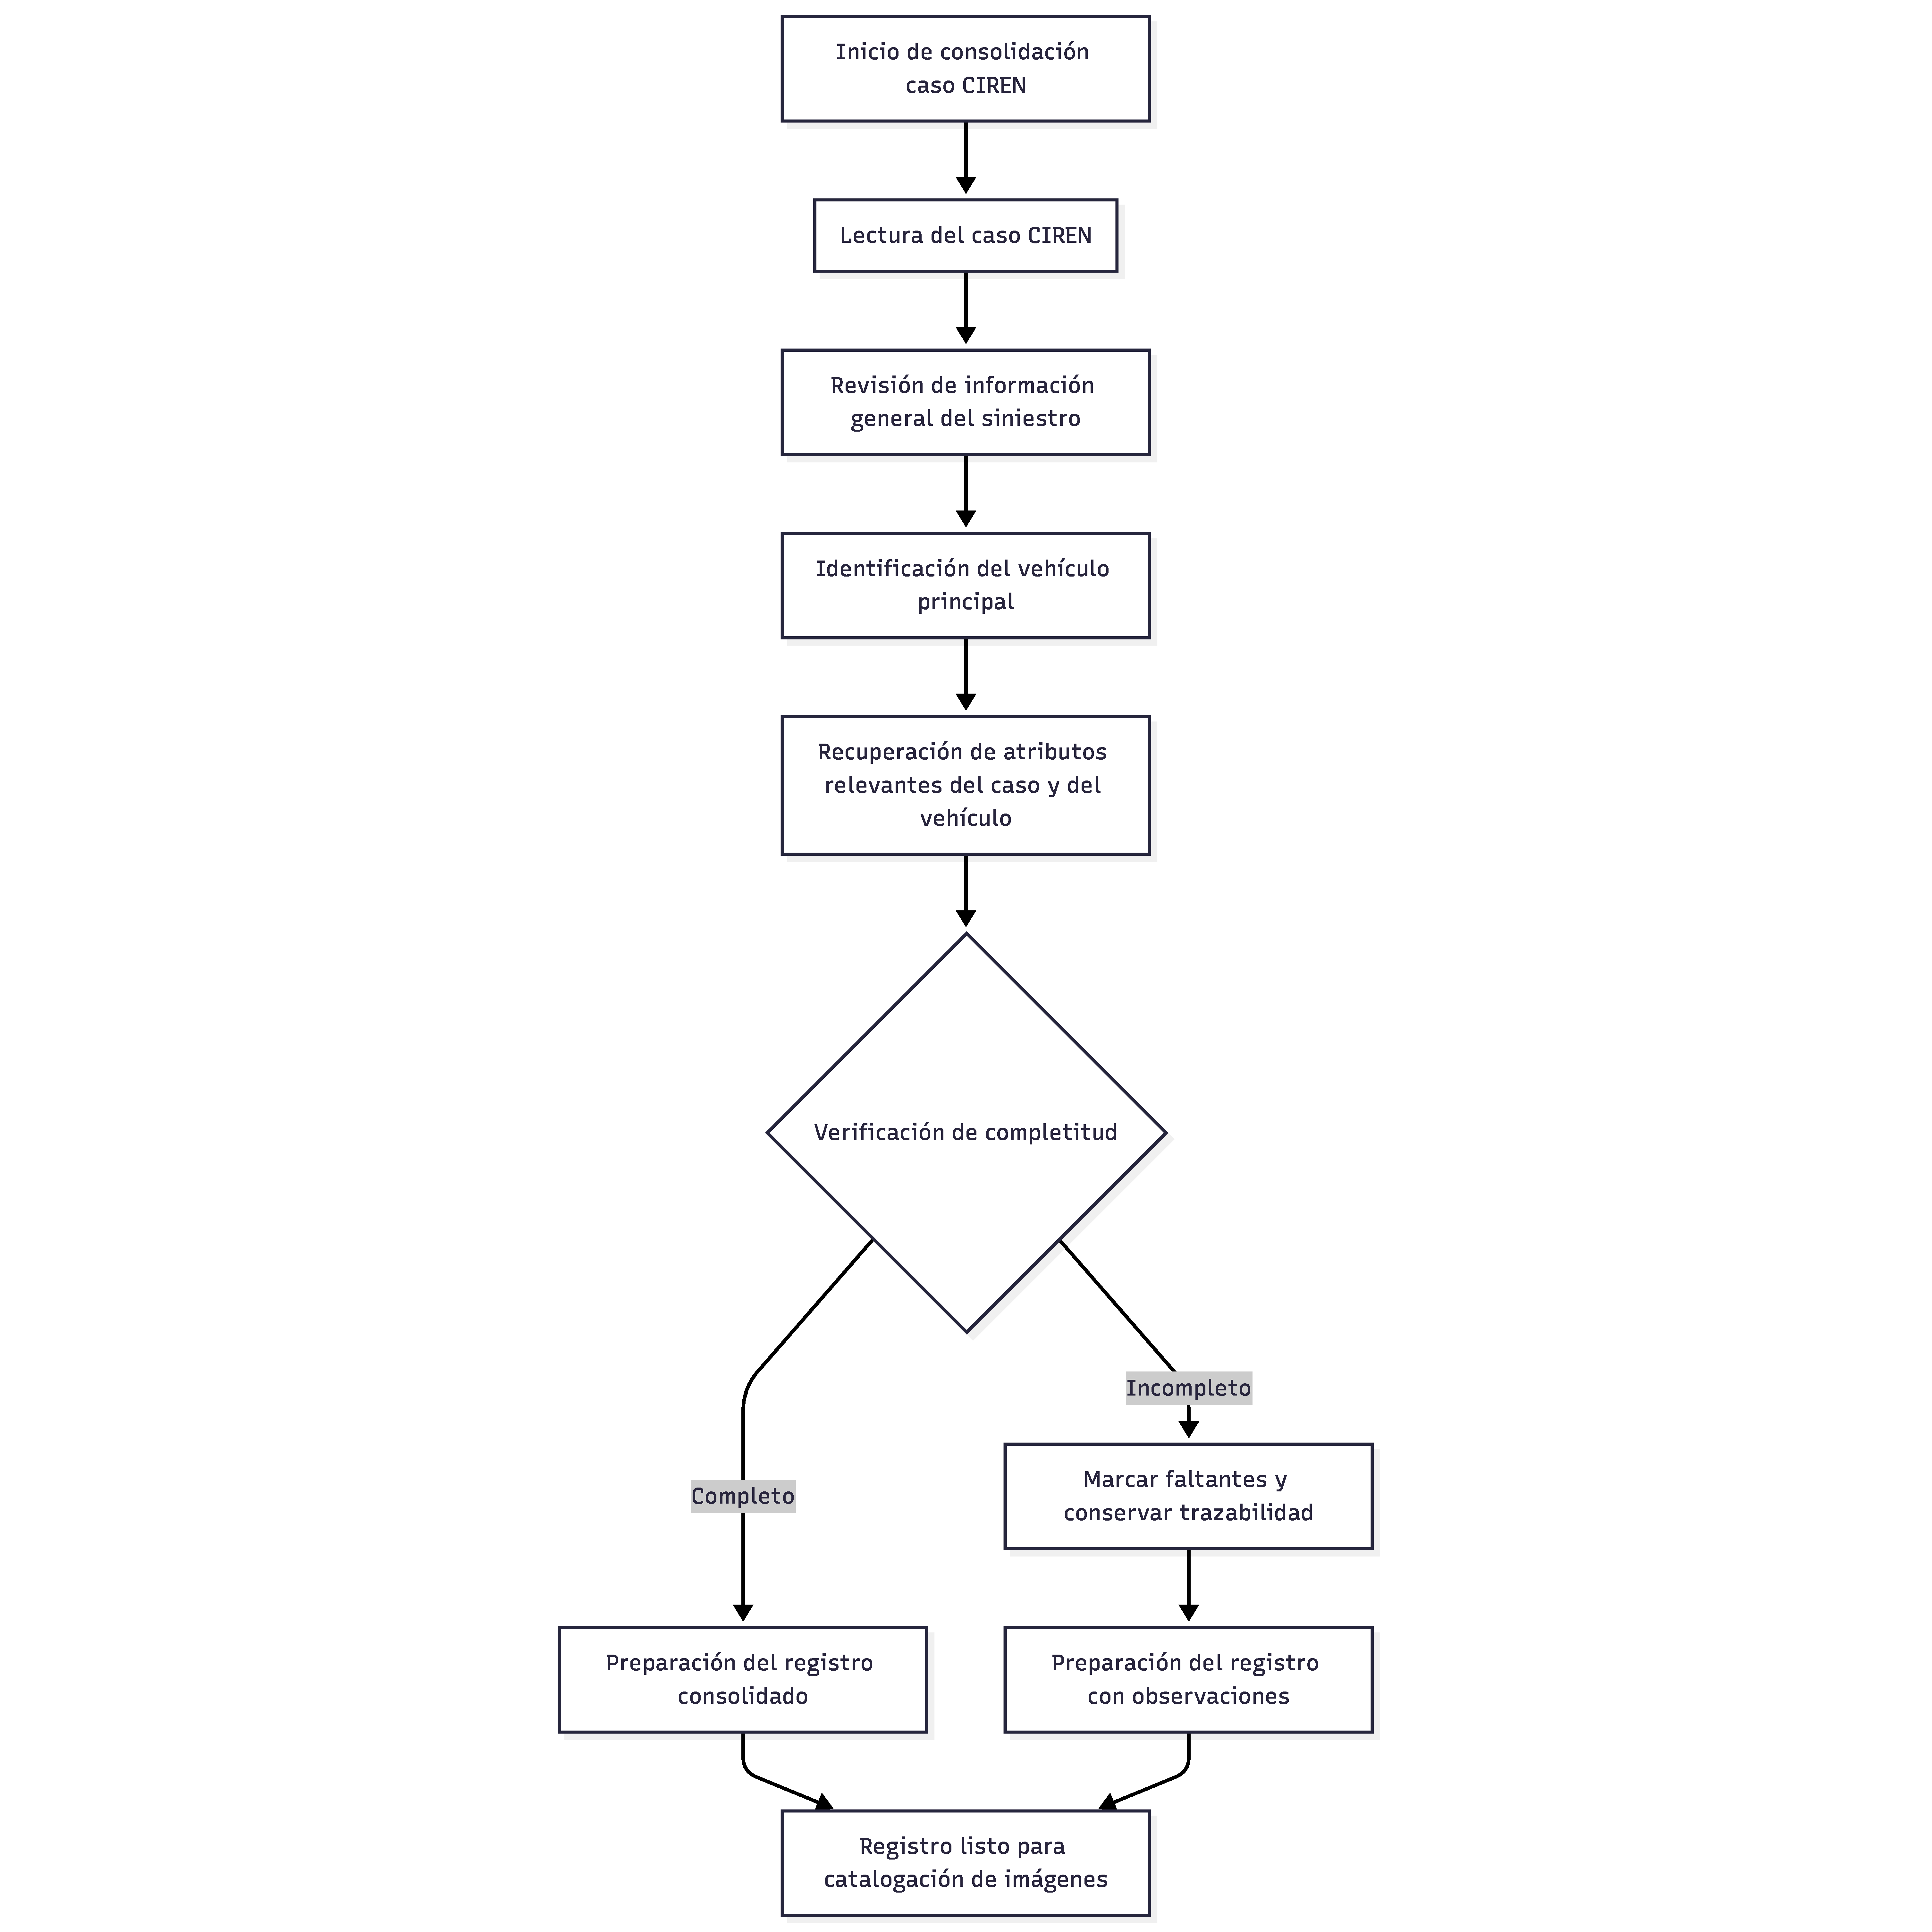
\includegraphics[width=\columnwidth]{Diagrams/Diagrama2.pdf}
    \caption{Diagrama de flujo que muestra la lógica de consolidación de un caso reportado en CIREN}
    \label{fig:diagrama1}
\end{figure}

\subsubsection{Catalogación de imágenes candidatas}

La colección fotográfica asociada a cada caso no se incorpora de manera directa a la base de datos final, sino que se lleva a cabo una fase de catalogación cuyo objetivo es reunir todas las vistas potencialmente útiles del vehículo seleccionado y registrar su procedencia. En esta etapa, cada imagen candidata conserva información descriptiva suficiente para identificarla posteriormente, incluyendo su relación con el vehículo, la vista o categoría visual de la que proviene y un identificador estable y estrictamente incremental para evitar la sobrescritura de archivos en tiempo de ejecución.

Metodológicamente, esta fase cumple dos funciones, la primera es separar el descubrimiento de contenido de la validación visual, lo cual reduce reprocesamiento en ejecuciones sucesivas y la segunda es imponer una preselección semántica: se descartan categorías de imágenes que típicamente aportan poco a la reconstrucción del daño estructural como lo pueden ser: tomas irrelevantes que no pertenezcan directamente a los vehículos involucrados, vistas no exteriores del automóvil o material complementario de baja utilidad para análisis forense del vehículo. Consecuentemente, el conjunto candidato se concentra en fotografías con mayor probabilidad de contener evidencia visual de interés.

\begin{figure}[htbp]
    \centering
    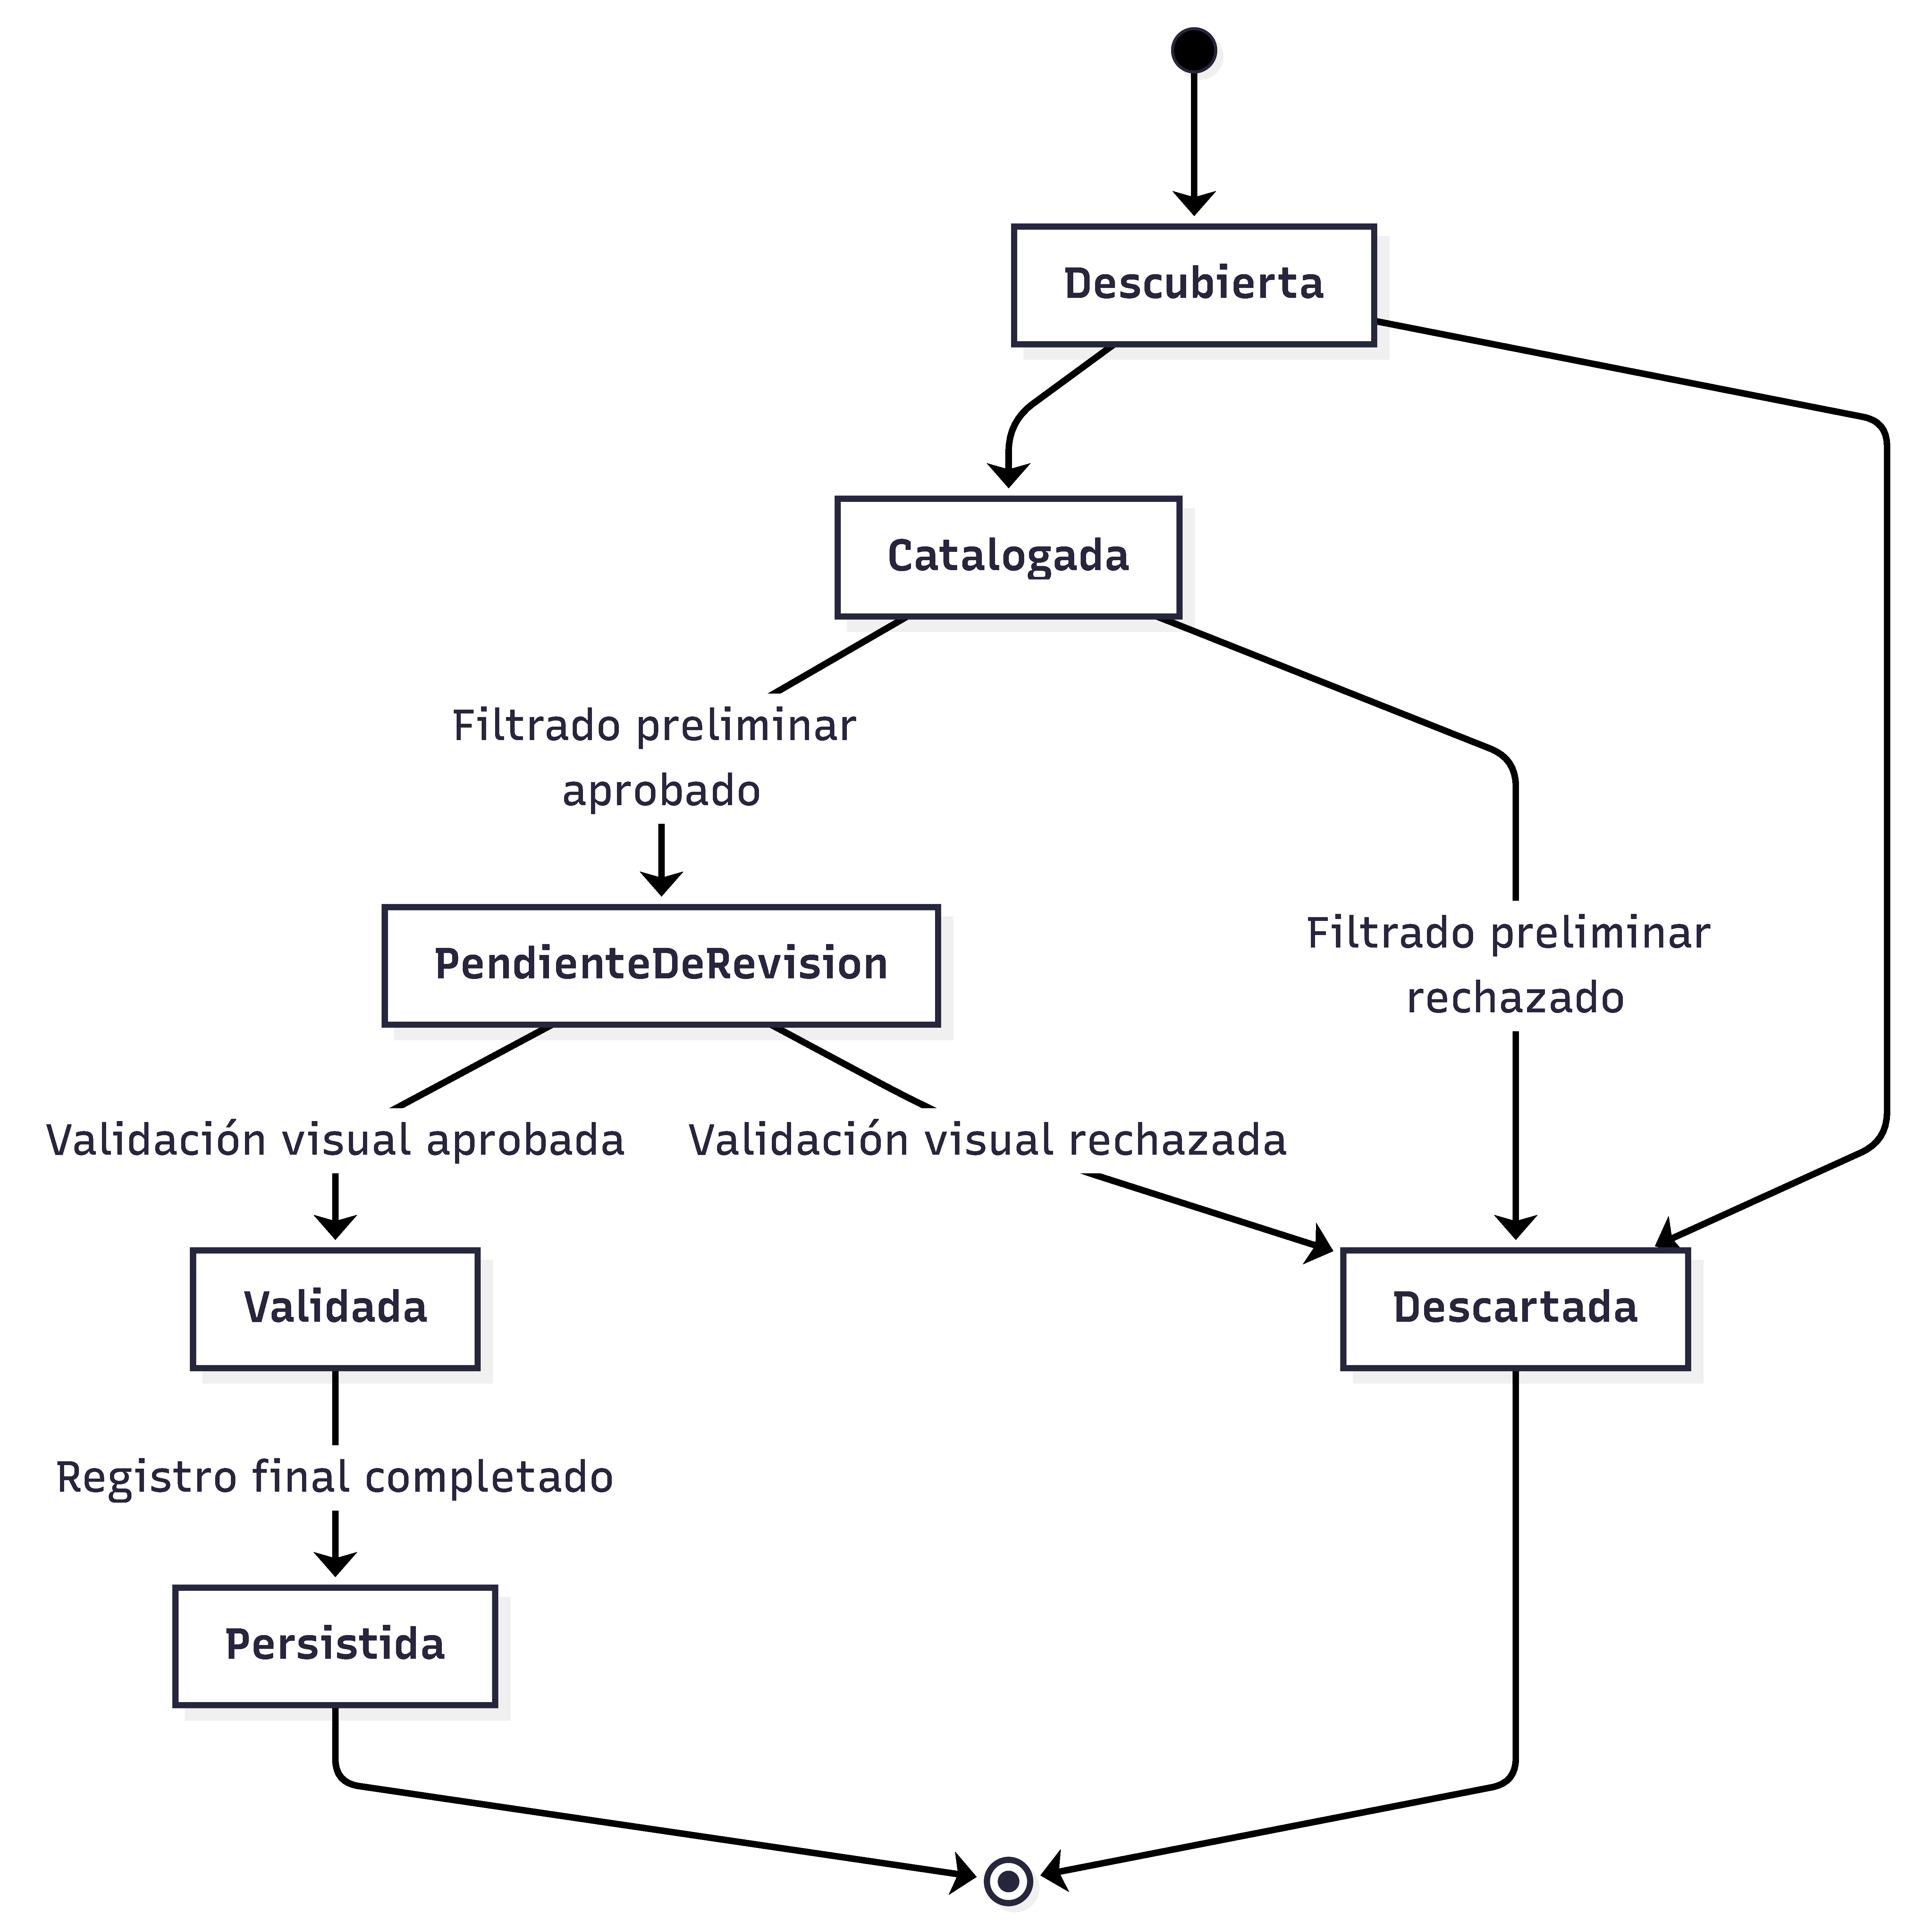
\includegraphics[width=\columnwidth]{Diagrams/Diagrama3.pdf}
    \caption{Diagrama de estados que muestra la transición de una imagen candidata a persistida o descartada}
    \label{fig:diagrama1}
\end{figure}

\subsubsection{Filtrado visual y validación de evidencia dañada}

Después de la catalogación, cada candidato se somete a una etapa de validación visual artificial orientada a confirmar que la fotografía contiene evidencia utilizable de daño vehicular. La lógica de esta etapa se centra en evitar que la base de datos final contenga imágenes sin daño apreciable o con contenido visual poco representativo del fenómeno de interés. Dicho de otro modo, no toda imagen asociada a un caso CIREN es útil para modelar severidad de colisión o estimar velocidad preimpacto. Por ello, fue necesario incorporar un filtro automatizado que priorice señales visibles de deformación estructural para reducir la probabilidad de ocurrencia de esta serie de casos innecesarios.

\begin{figure}[htbp]
    \centering
    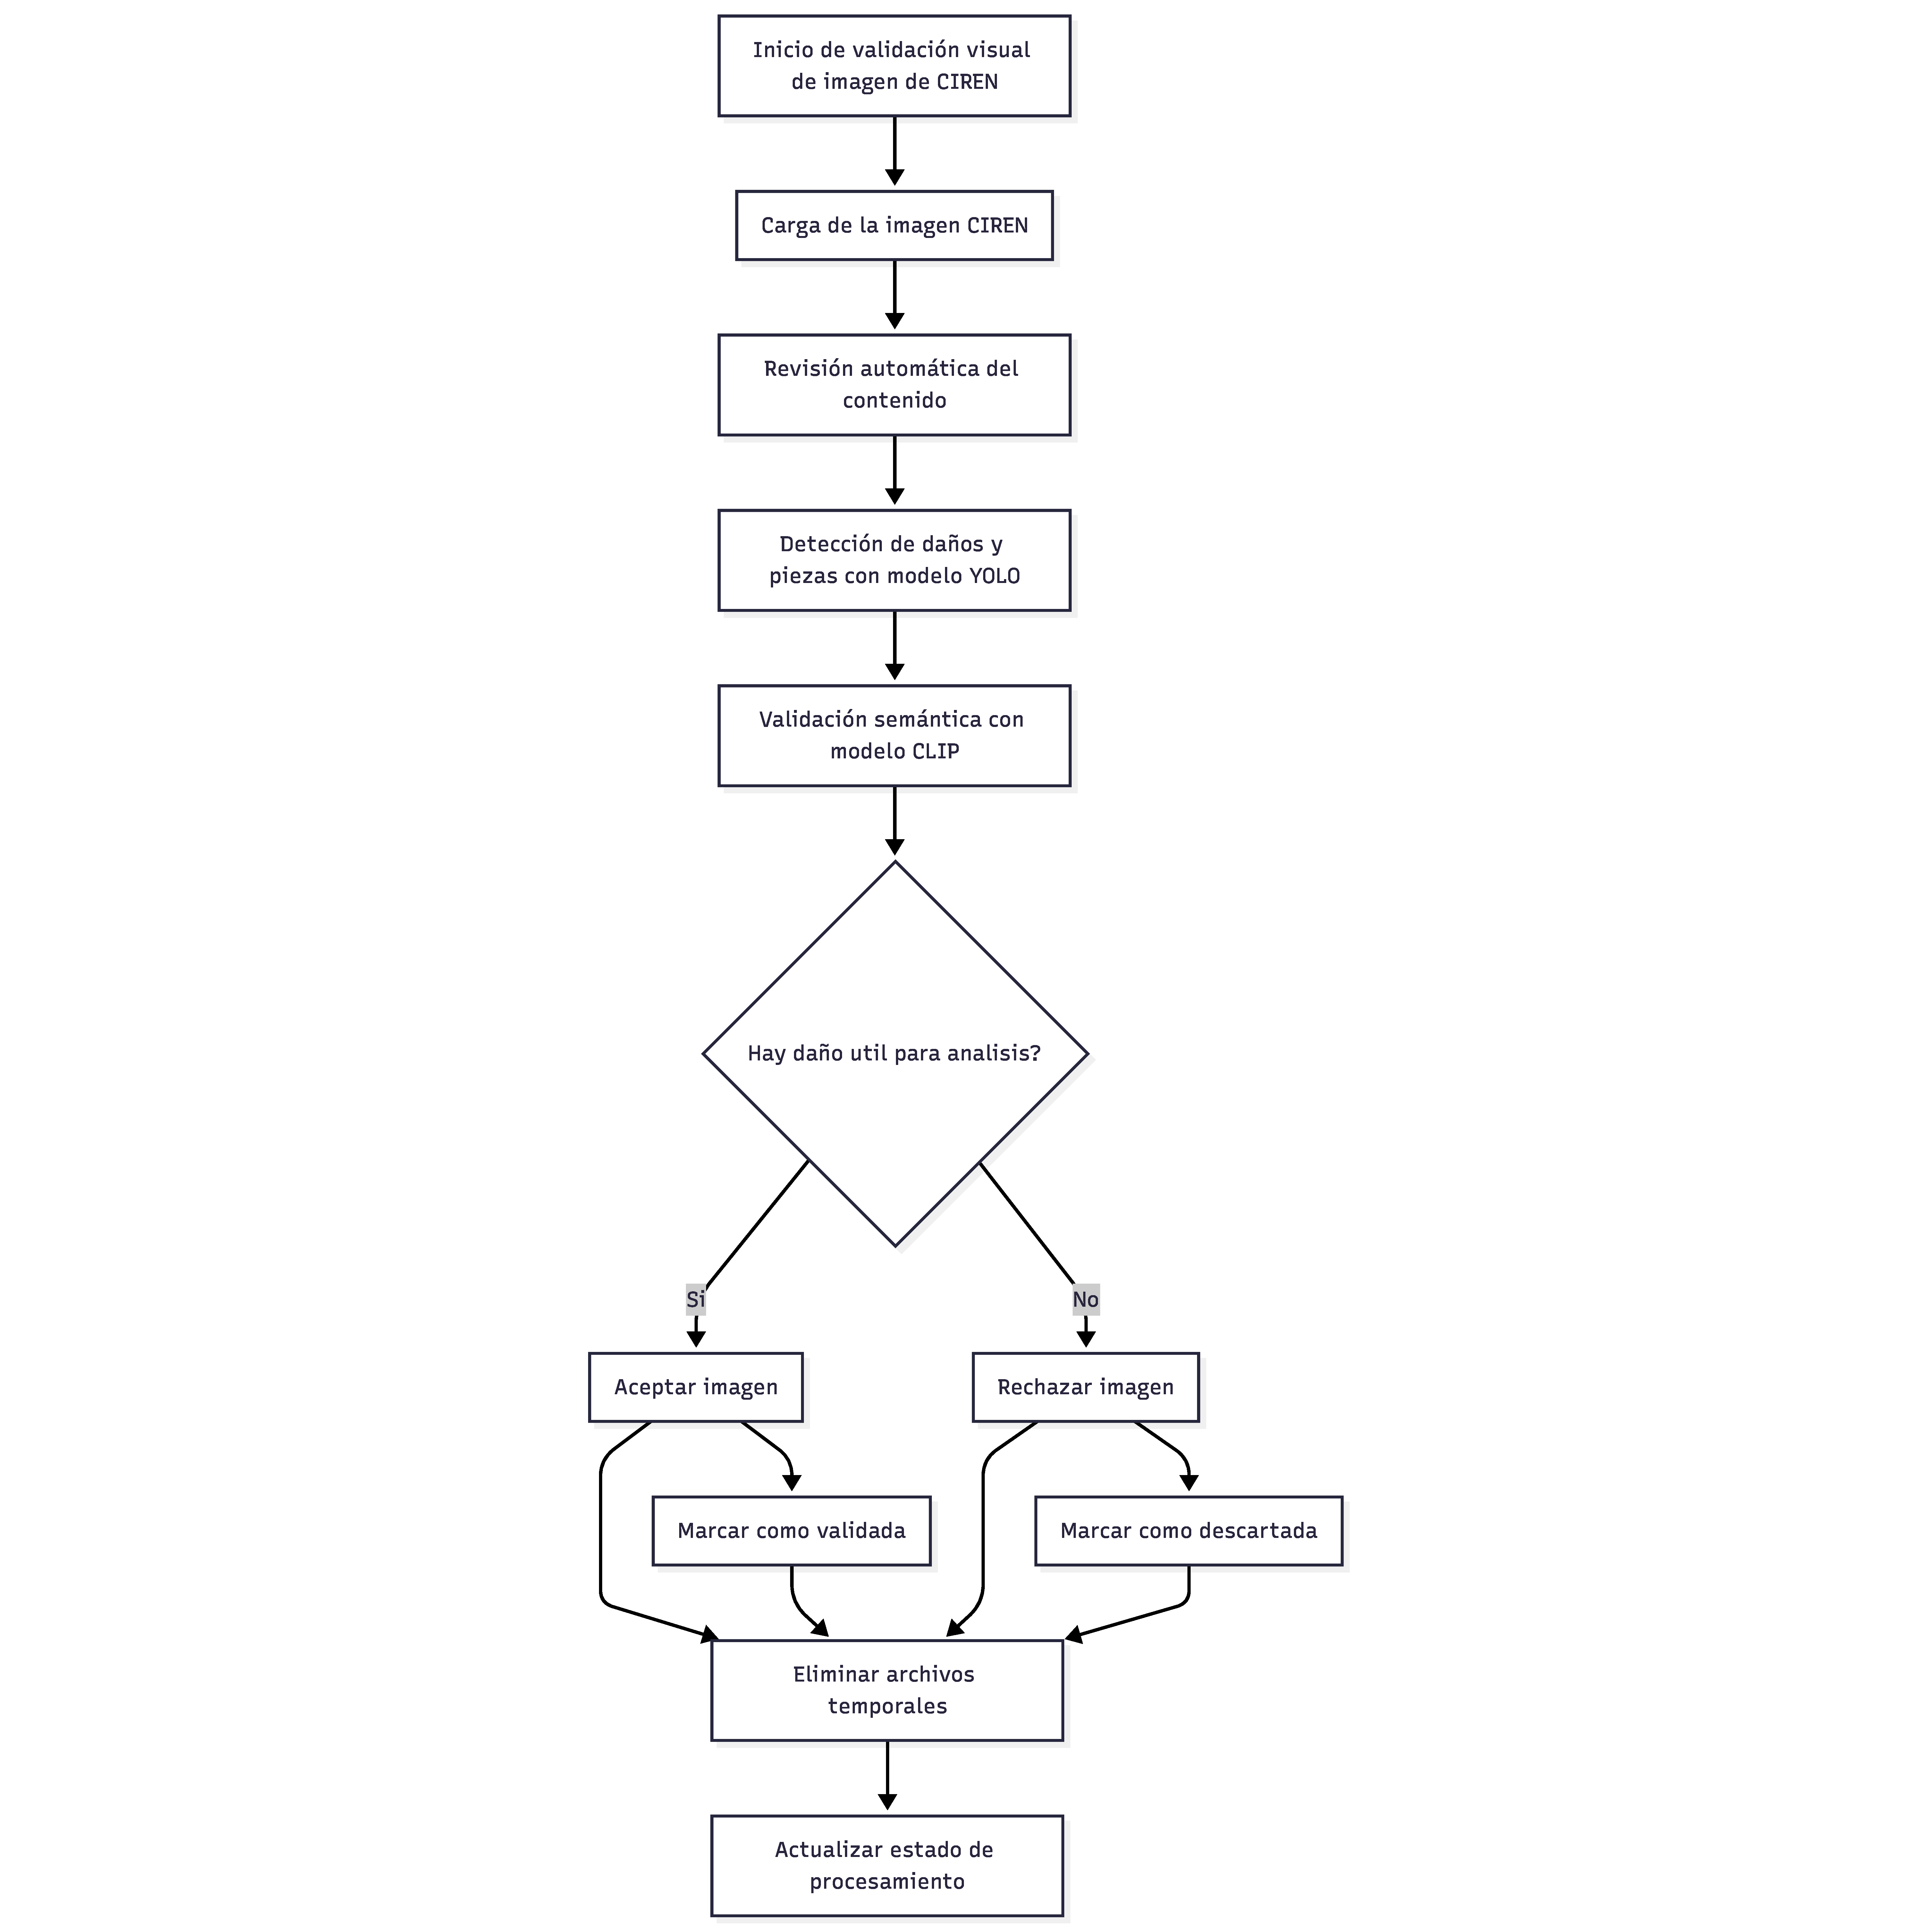
\includegraphics[width=\columnwidth]{Diagrams/Diagrama4.pdf}
    \caption{Diagrama de flujo donde se muestra el proceso de validación visual de una imagen extraída de un caso en CIREN}
    \label{fig:diagrama1}
\end{figure}


\subsubsection{Normalización de salidas para análisis posterior}

El resultado del preprocesamiento de imágenes y características extraídas desde CIREN es organizado en dos niveles complementarios: caso e imagen. El primero se concentra en la caracterización del siniestro y del vehículo, mientras que el segundo tiene el objetivo de conservar la evidencia visual validada con su referencia al caso correspondiente. Esta separación permite analizar la información desde una perspectiva estadística o computacional sin perder la granularidad particular de cada fotografía.

\begin{figure}[htbp]
    \centering
    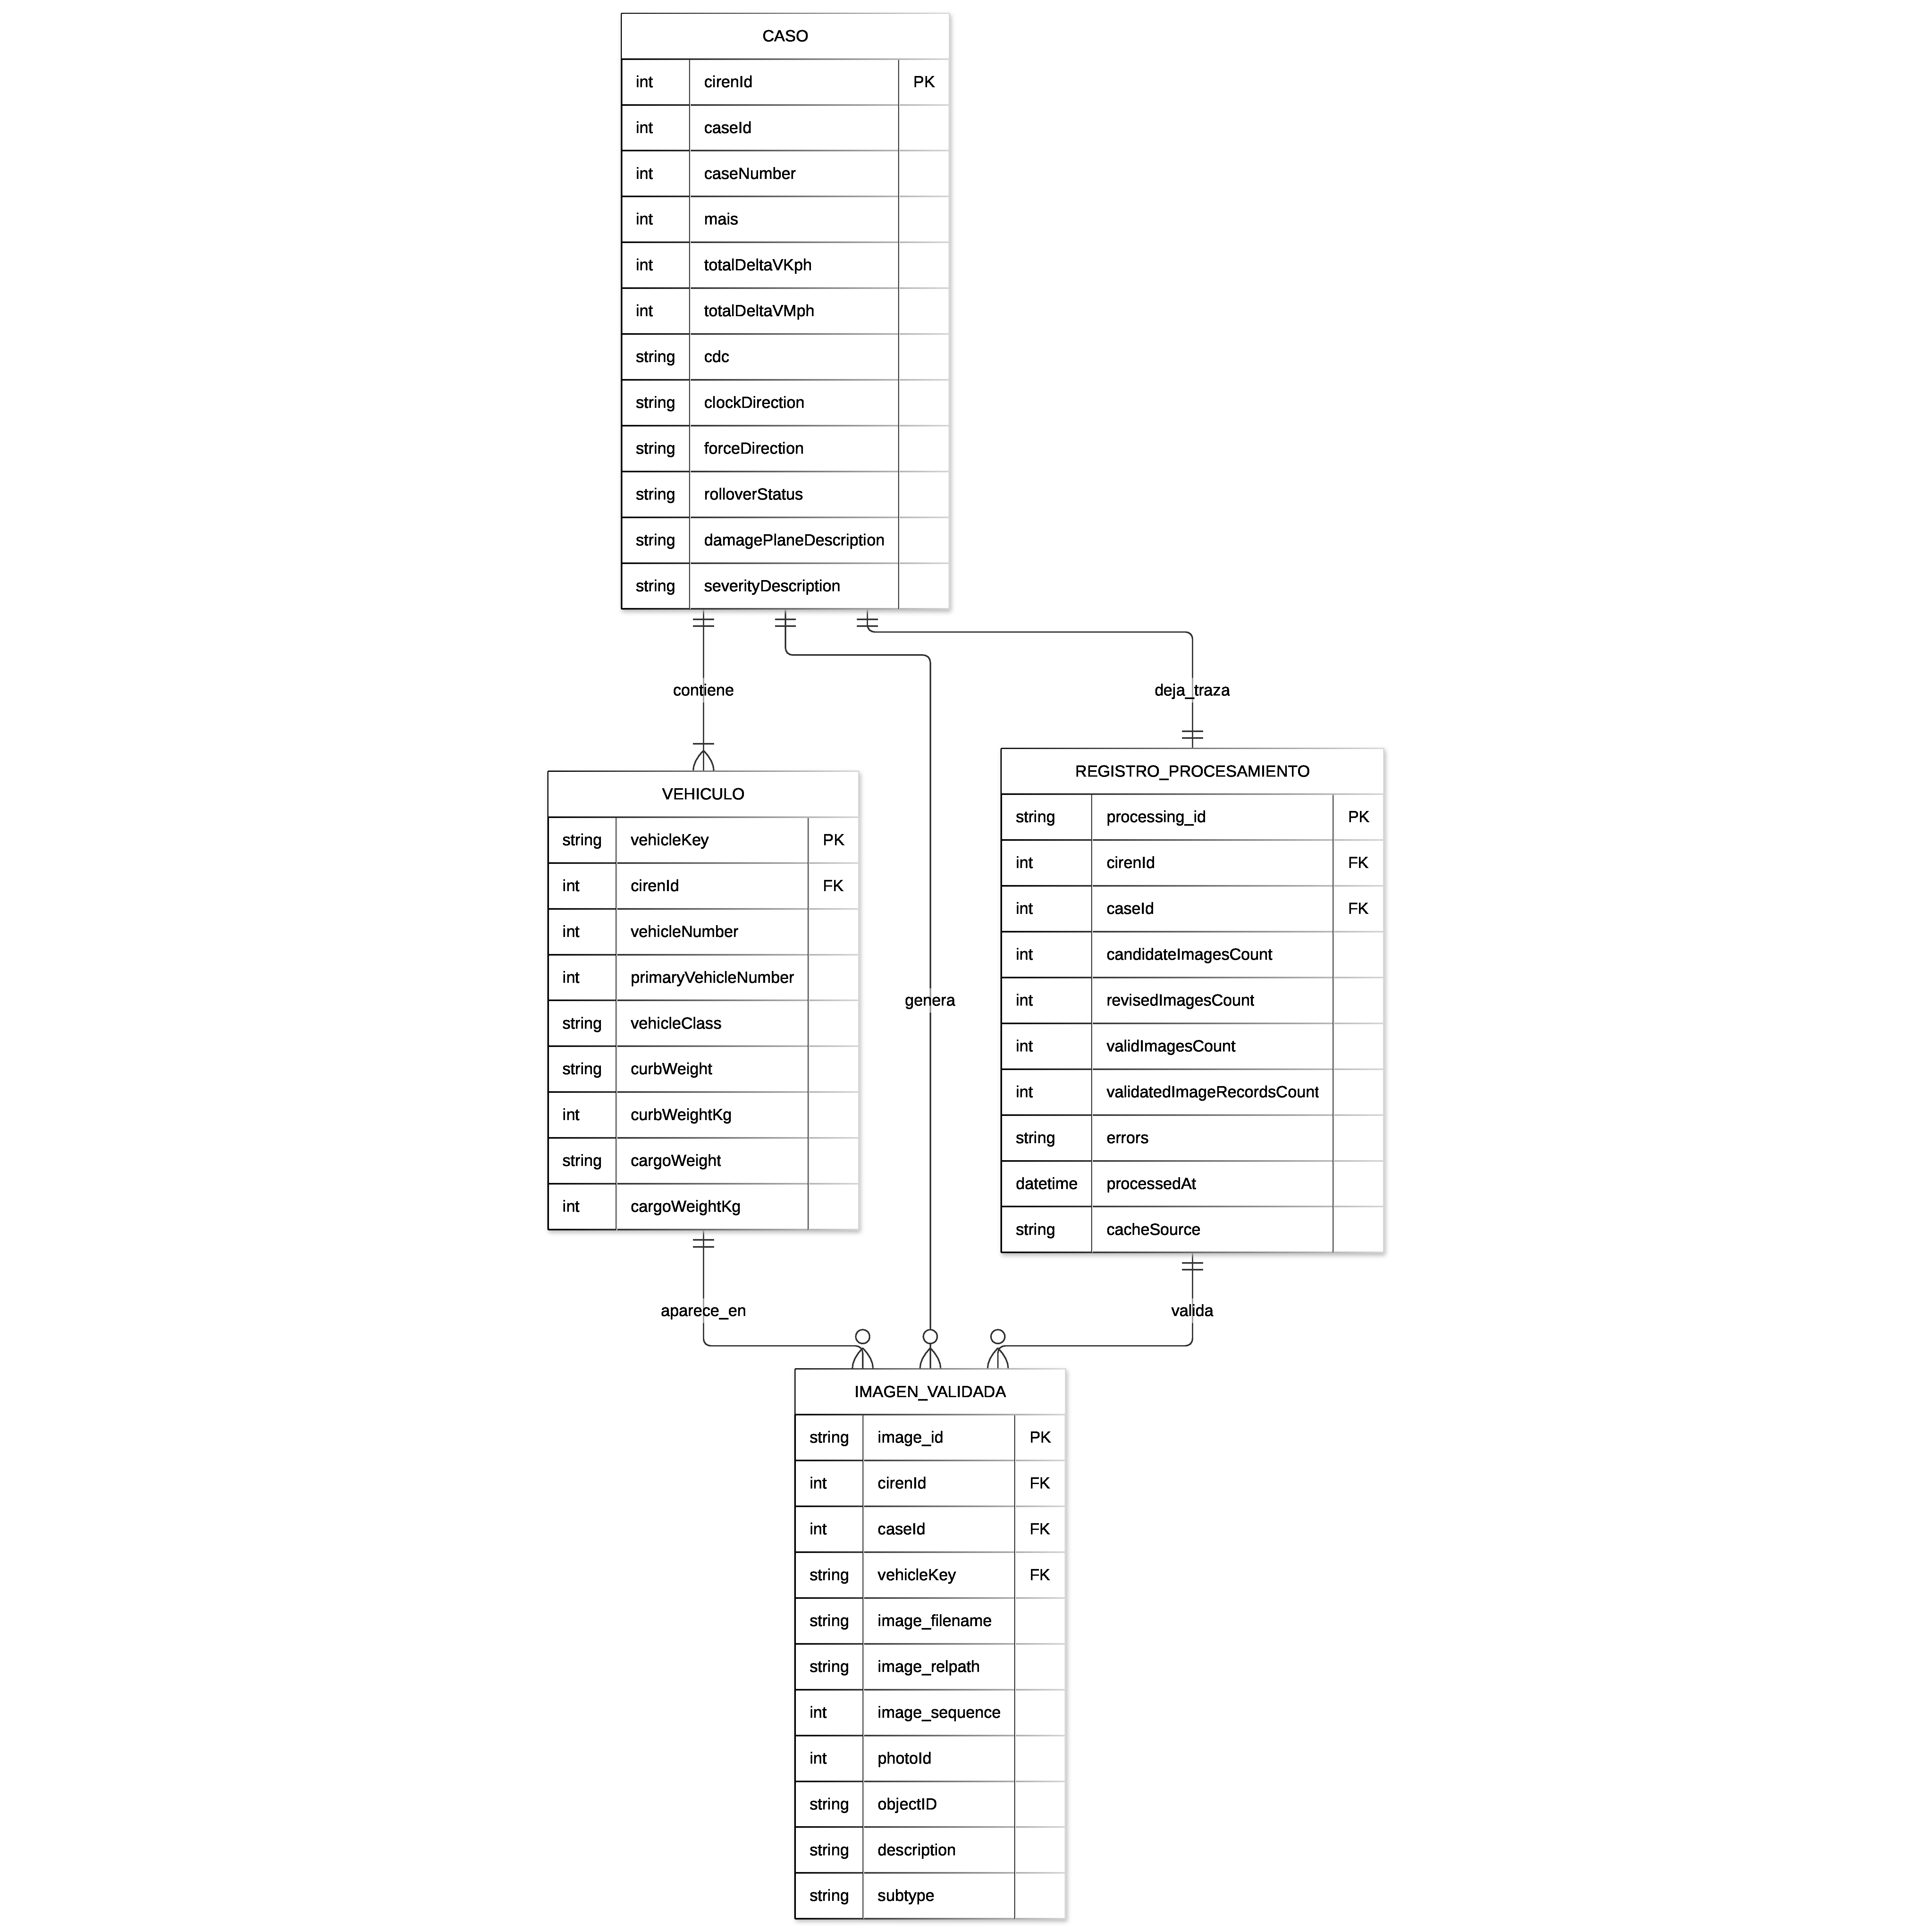
\includegraphics[width=\columnwidth]{Diagrams/Diagrama7.pdf}
    \caption{Diagrama de entidad relación del conjunto resultante del preprocesamiento y extracción de datos de CIREN}
    \label{fig:diagrama1}
\end{figure}

\subsection{Preprocesamiento de la base de datos alojada en HuggingFace para el entrenamiento de los modelos}
El preprocesamiento del dataset se realizó mediante un flujo estructurado basado en scikit-learn, diseñado para limpiar las observaciones, separar la variable objetivo (totalDeltaVKph) y transformar cada tipo de atributo de acuerdo con su naturaleza. En una primera etapa, se eliminaron los registros con valores nulos en la variable objetivo y se excluyeron columnas no informativas para el modelado. Posteriormente, se aplicó un ColumnTransformer con transformaciones específicas: las variables numéricas relacionadas con peso fueron imputadas con la mediana y estandarizadas; las variables categóricas nominales se imputaron con una categoría genérica y se codificaron mediante one-hot encoding; la severidad se trató como variable ordinal respetando un orden predefinido; el valor mais se procesó extrayendo su componente numérico antes de imputar y escalar; y las direcciones angulares (forceDirection y clockDirection) se convirtieron a representaciones cíclicas mediante seno y coseno para preservar su periodicidad. Finalmente, el estado de volcadura se binarizó en una variable indicadora. Este procedimiento permitió obtener una matriz de características numérica, consistente y apta para el entrenamiento de modelos de regresión orientados a estimar la velocidad de impacto.

\subsection{Arquitectura propuesta}
Nam nec ante. Sed lacinia, urna non tincidunt mattis, tortor neque adipiscing diam, a cursus ipsum ante quis turpis. Nulla facilisi. Ut fringilla. Suspendisse potenti. Nunc feugiat mi a tellus consequat imperdiet.

\section{RESULTADOS}
Lorem ipsum dolor sit amet, consectetur adipiscing elit. Pellentesque nibh. Aenean quam. In scelerisque sem at dolor. Maecenas mattis. Sed convallis tristique sem. Proin ut ligula vel nunc egestas porttitor. Morbi lectus risus, iaculis vel, suscipit quis, luctus non, massa.

Fusce ac turpis quis ligula lacinia aliquet. Mauris ipsum. Nulla metus metus, ullamcorper vel, tincidunt sed, euismod in, nibh. Quisque volutpat condimentum velit. Class aptent taciti sociosqu ad litora torquent per conubia nostra.

Nam nec ante. Sed lacinia, urna non tincidunt mattis, tortor neque adipiscing diam, a cursus ipsum ante quis turpis. Nulla facilisi. Ut fringilla. Suspendisse potenti. Nunc feugiat mi a tellus consequat imperdiet.

Vestibulum sapien. Proin quam. Etiam ultrices. Suspendisse in justo eu magna luctus suscipit. Sed lectus. Integer euismod lacus luctus magna. Quisque cursus, metus vitae pharetra auctor, sem massa mattis sem.

\subsection{Metricas cuantitativas}
Lorem ipsum dolor sit amet, consectetur adipiscing elit. Sed do eiusmod tempor incididunt ut labore et dolore magna aliqua. Ut enim ad minim veniam, quis nostrud exercitation ullamco laboris nisi ut aliquip ex ea commodo consequat.

\subsection{Analisis cualitativo}
Duis aute irure dolor in reprehenderit in voluptate velit esse cillum dolore eu fugiat nulla pariatur. Excepteur sint occaecat cupidatat non proident, sunt in culpa qui officia deserunt mollit anim id est laborum.

\section{DISCUSIÓN}
Lorem ipsum dolor sit amet, consectetur adipiscing elit. Sed do eiusmod tempor incididunt ut labore et dolore magna aliqua. Ut enim ad minim veniam, quis nostrud exercitation ullamco laboris nisi ut aliquip ex ea commodo consequat. Duis aute irure dolor in reprehenderit in voluptate velit esse cillum dolore eu fugiat nulla pariatur.

Excepteur sint occaecat cupidatat non proident, sunt in culpa qui officia deserunt mollit anim id est laborum. Sed ut perspiciatis unde omnis iste natus error sit voluptatem accusantium doloremque laudantium. Totam rem aperiam, eaque ipsa quae ab illo inventore veritatis et quasi architecto beatae vitae dicta sunt explicabo.

Nemo enim ipsam voluptatem quia voluptas sit aspernatur aut odit aut fugit. Sed quia consequuntur magni dolores eos qui ratione voluptatem sequi nesciunt. Neque porro quisquam est, qui dolorem ipsum quia dolor sit amet.

\subsection{Interpretacion de hallazgos}
Lorem ipsum dolor sit amet, consectetur adipiscing elit. Integer nec odio. Praesent libero. Sed cursus ante dapibus diam. Sed nisi. Nulla quis sem at nibh elementum imperdiet.

\subsection{Limitaciones}
Duis sagittis ipsum. Praesent mauris. Fusce nec tellus sed augue semper porta. Mauris massa. Vestibulum lacinia arcu eget nulla. Class aptent taciti sociosqu ad litora torquent per conubia nostra.

\section{CONCLUSIONES}
Lorem ipsum dolor sit amet, consectetur adipiscing elit. Proin quam. Etiam ultrices. Suspendisse in justo eu magna luctus suscipit. Sed lectus. Integer euismod lacus luctus magna.

\subsection{Resumen final}
Lorem ipsum dolor sit amet, consectetur adipiscing elit. Sed do eiusmod tempor incididunt ut labore et dolore magna aliqua. Ut enim ad minim veniam, quis nostrud exercitation ullamco laboris nisi ut aliquip ex ea commodo consequat.

\subsection{Trabajo futuro}
Duis aute irure dolor in reprehenderit in voluptate velit esse cillum dolore eu fugiat nulla pariatur. Excepteur sint occaecat cupidatat non proident, sunt in culpa qui officia deserunt mollit anim id est laborum.

% Referencias o fuentes bibliograficas
\insertbibliography{References}

\end{document}
